% Options for packages loaded elsewhere
\PassOptionsToPackage{unicode}{hyperref}
\PassOptionsToPackage{hyphens}{url}
%
\documentclass[
]{book}
\title{The intersection of business and biology}
\author{Tobin Turner}
\date{2022-03-22}

\usepackage{amsmath,amssymb}
\usepackage{lmodern}
\usepackage{iftex}
\ifPDFTeX
  \usepackage[T1]{fontenc}
  \usepackage[utf8]{inputenc}
  \usepackage{textcomp} % provide euro and other symbols
\else % if luatex or xetex
  \usepackage{unicode-math}
  \defaultfontfeatures{Scale=MatchLowercase}
  \defaultfontfeatures[\rmfamily]{Ligatures=TeX,Scale=1}
\fi
% Use upquote if available, for straight quotes in verbatim environments
\IfFileExists{upquote.sty}{\usepackage{upquote}}{}
\IfFileExists{microtype.sty}{% use microtype if available
  \usepackage[]{microtype}
  \UseMicrotypeSet[protrusion]{basicmath} % disable protrusion for tt fonts
}{}
\makeatletter
\@ifundefined{KOMAClassName}{% if non-KOMA class
  \IfFileExists{parskip.sty}{%
    \usepackage{parskip}
  }{% else
    \setlength{\parindent}{0pt}
    \setlength{\parskip}{6pt plus 2pt minus 1pt}}
}{% if KOMA class
  \KOMAoptions{parskip=half}}
\makeatother
\usepackage{xcolor}
\IfFileExists{xurl.sty}{\usepackage{xurl}}{} % add URL line breaks if available
\IfFileExists{bookmark.sty}{\usepackage{bookmark}}{\usepackage{hyperref}}
\hypersetup{
  pdftitle={The intersection of business and biology},
  pdfauthor={Tobin Turner},
  hidelinks,
  pdfcreator={LaTeX via pandoc}}
\urlstyle{same} % disable monospaced font for URLs
\usepackage{longtable,booktabs,array}
\usepackage{calc} % for calculating minipage widths
% Correct order of tables after \paragraph or \subparagraph
\usepackage{etoolbox}
\makeatletter
\patchcmd\longtable{\par}{\if@noskipsec\mbox{}\fi\par}{}{}
\makeatother
% Allow footnotes in longtable head/foot
\IfFileExists{footnotehyper.sty}{\usepackage{footnotehyper}}{\usepackage{footnote}}
\makesavenoteenv{longtable}
\usepackage{graphicx}
\makeatletter
\def\maxwidth{\ifdim\Gin@nat@width>\linewidth\linewidth\else\Gin@nat@width\fi}
\def\maxheight{\ifdim\Gin@nat@height>\textheight\textheight\else\Gin@nat@height\fi}
\makeatother
% Scale images if necessary, so that they will not overflow the page
% margins by default, and it is still possible to overwrite the defaults
% using explicit options in \includegraphics[width, height, ...]{}
\setkeys{Gin}{width=\maxwidth,height=\maxheight,keepaspectratio}
% Set default figure placement to htbp
\makeatletter
\def\fps@figure{htbp}
\makeatother
\setlength{\emergencystretch}{3em} % prevent overfull lines
\providecommand{\tightlist}{%
  \setlength{\itemsep}{0pt}\setlength{\parskip}{0pt}}
\setcounter{secnumdepth}{5}
\usepackage{booktabs}
\ifLuaTeX
  \usepackage{selnolig}  % disable illegal ligatures
\fi
\usepackage[]{natbib}
\bibliographystyle{apalike}

\begin{document}
\maketitle

{
\setcounter{tocdepth}{1}
\tableofcontents
}
\hypertarget{about}{%
\chapter{About}\label{about}}

This is a little talk about my interest in the intersection of business and biology.

\hypertarget{motivation}{%
\chapter{Motivation}\label{motivation}}

Like father, like daughter.

\begin{center}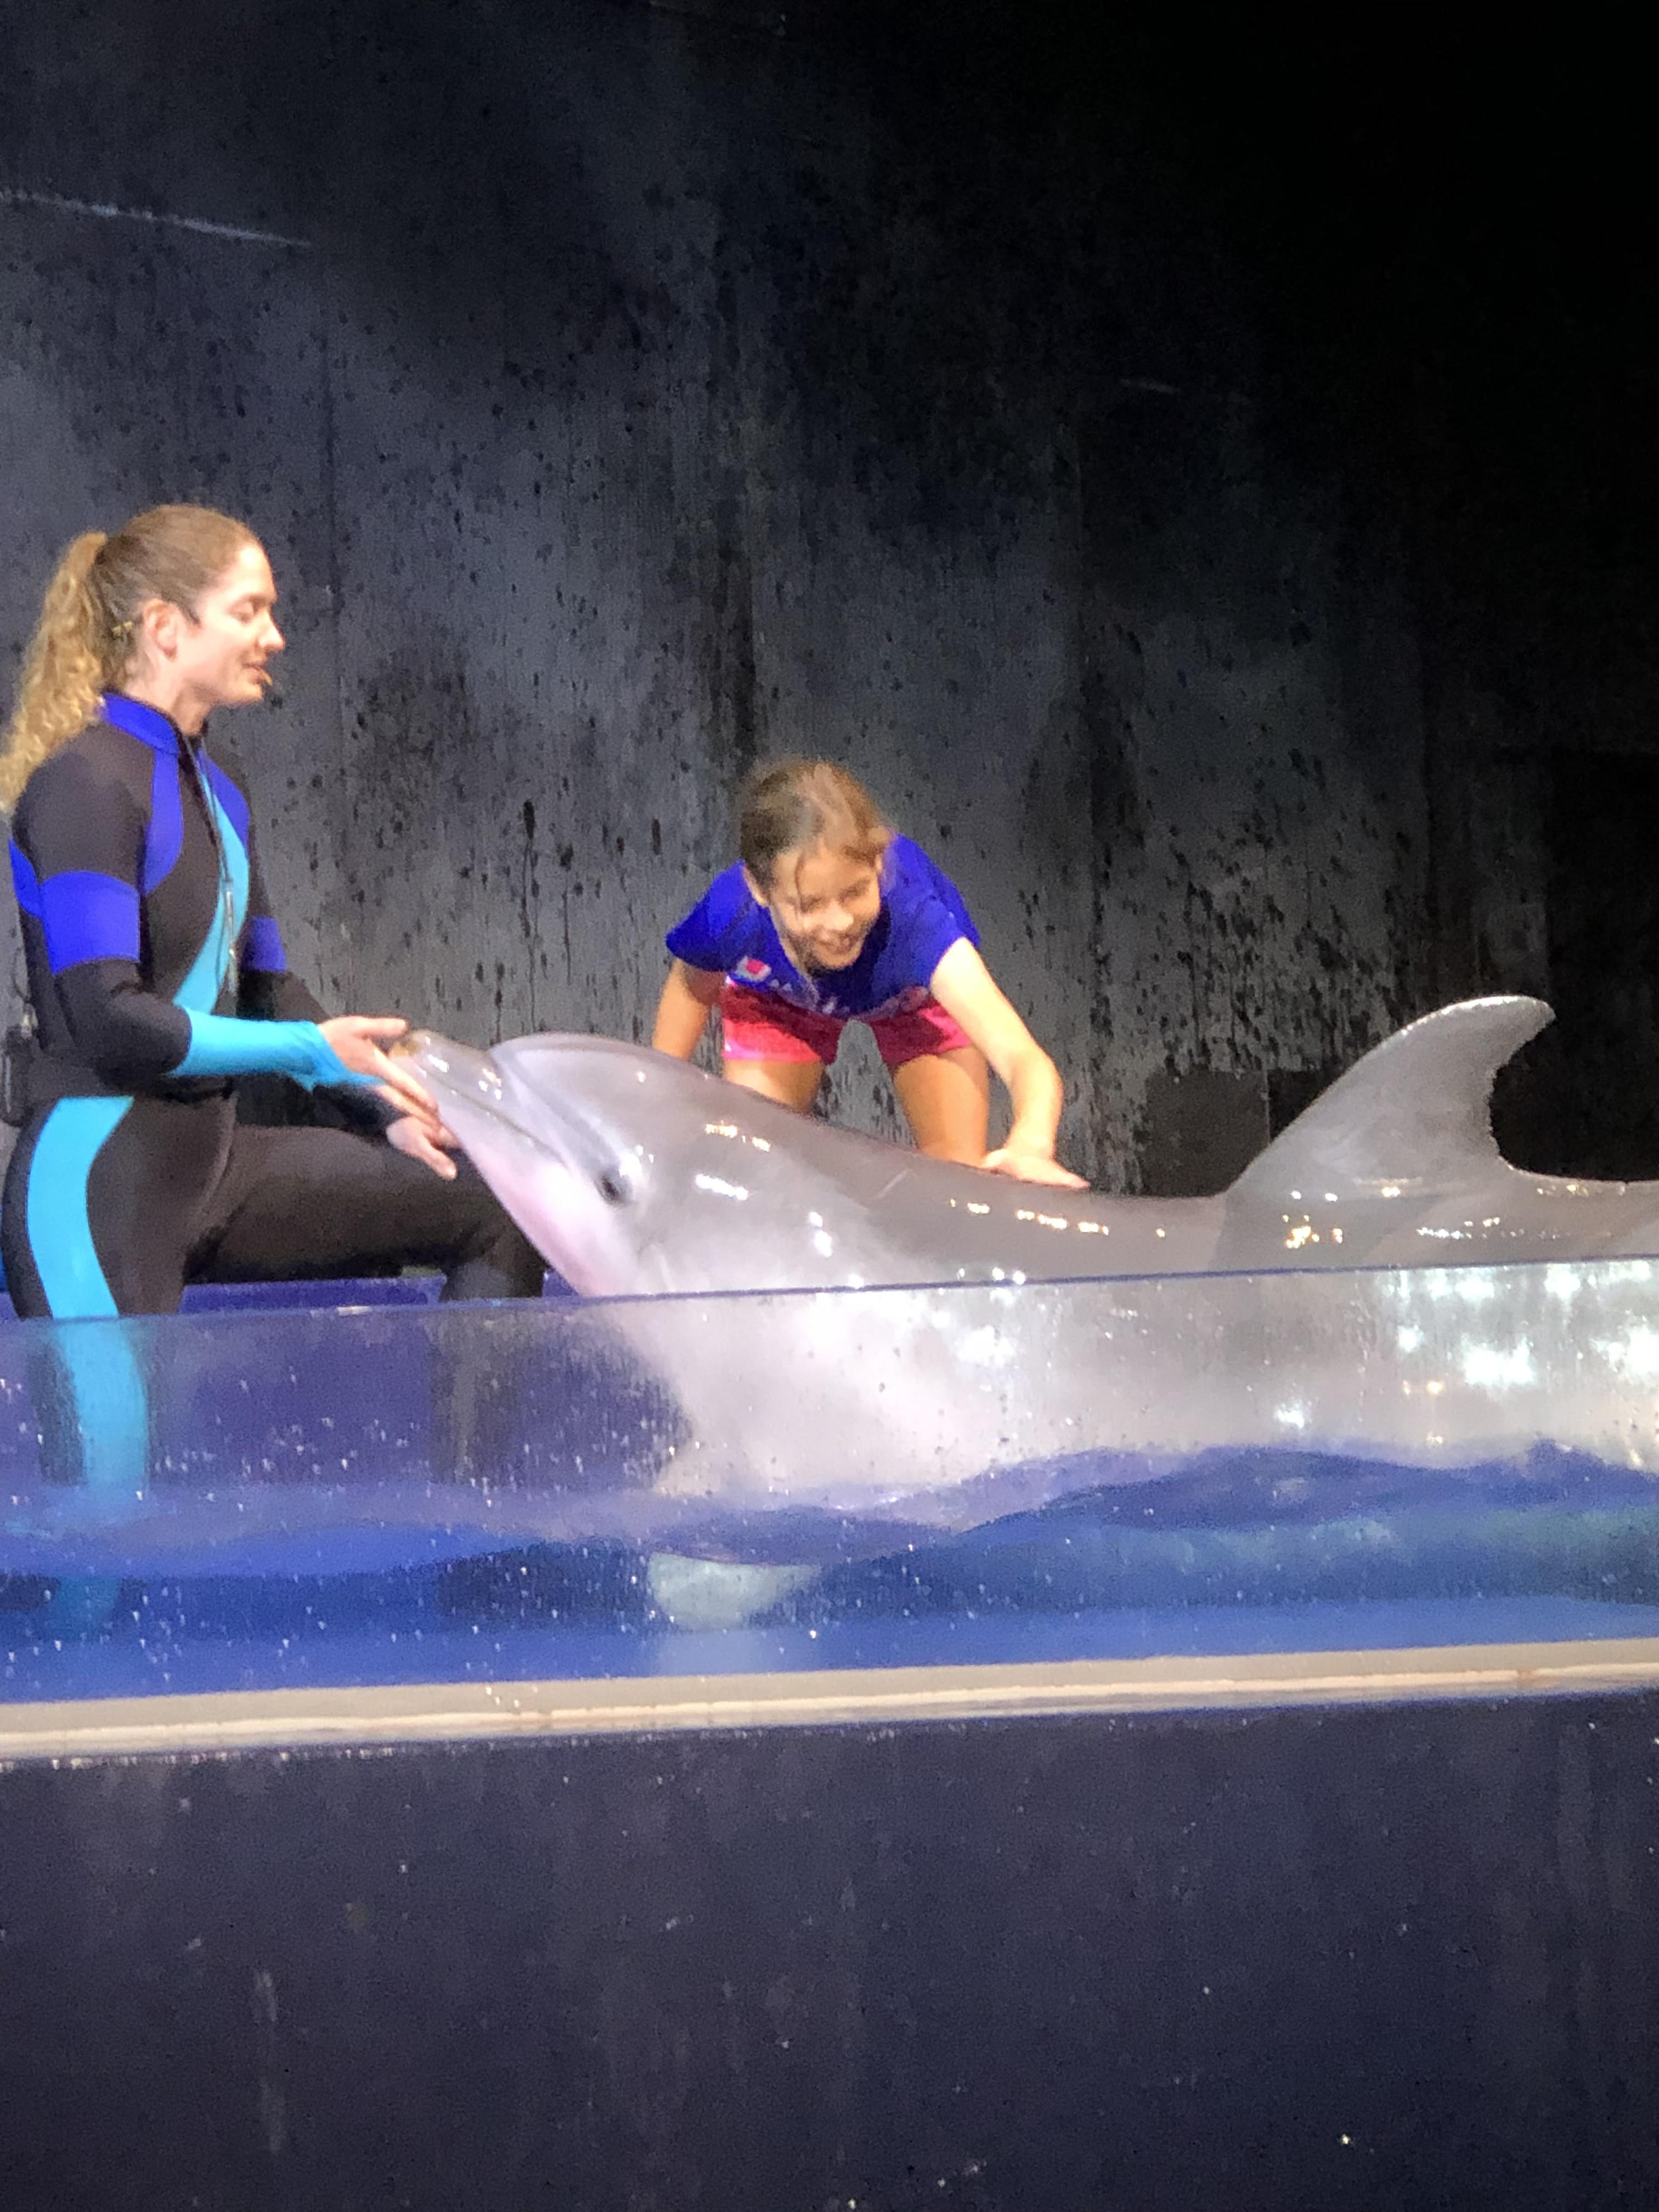
\includegraphics{_images/meredith} \end{center}

\hypertarget{an-unexpected-influence}{%
\chapter{An unexpected influence}\label{an-unexpected-influence}}

Bryce Stewart, PhD, University of York

\begin{center}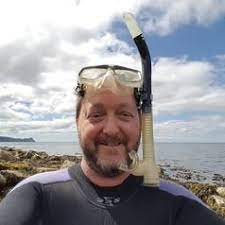
\includegraphics{_images/bryce} \end{center}

\hypertarget{real-life-case-study}{%
\chapter{Real life case study}\label{real-life-case-study}}

Living it out.

\begin{center}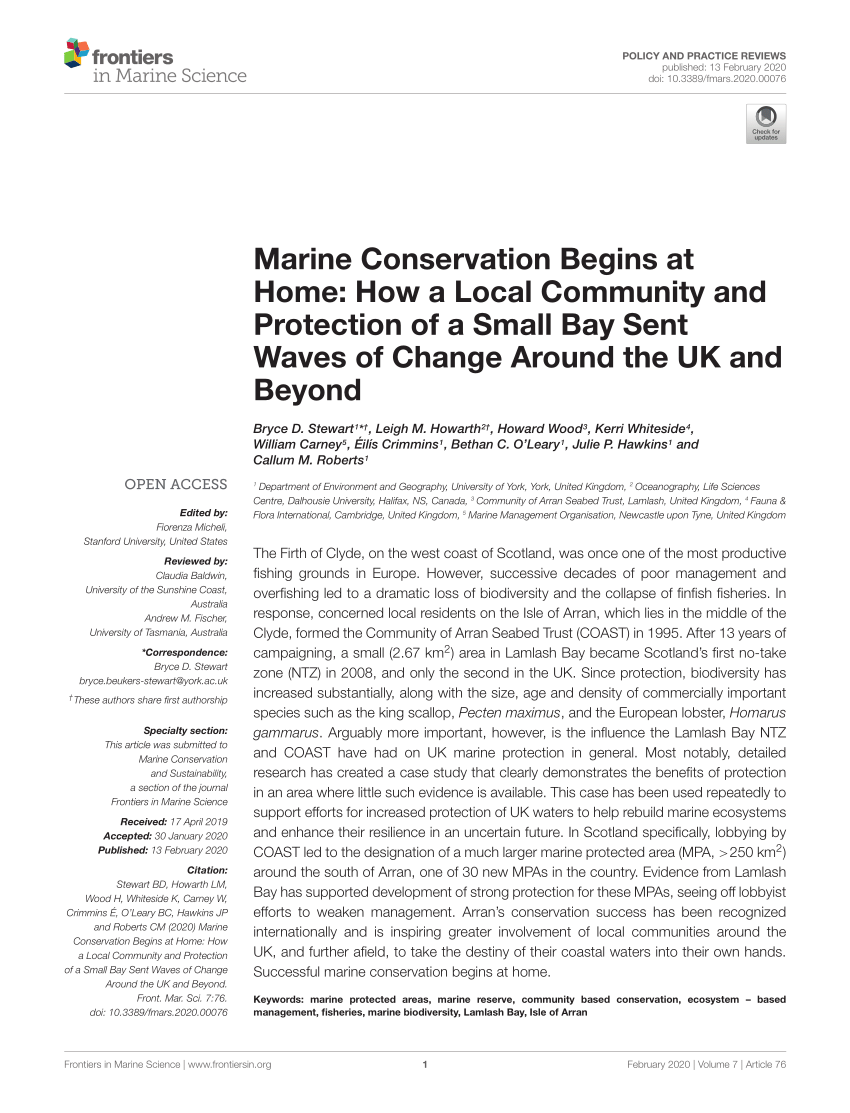
\includegraphics{_images/marine} \end{center}

:::

\hypertarget{the-importance-of-science-rigor}{%
\chapter{The importance of science, rigor}\label{the-importance-of-science-rigor}}

Study something you love. And that tastes great.

\begin{center}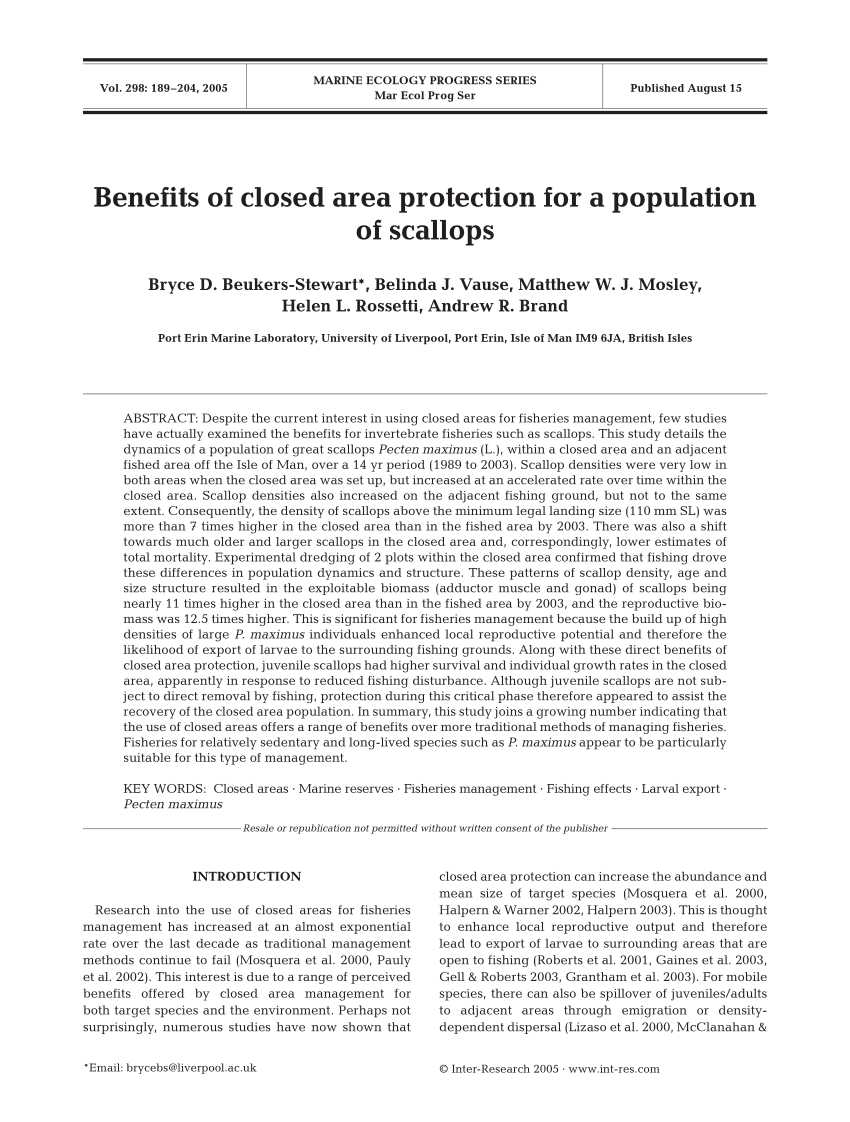
\includegraphics{_images/benefits} \end{center}

\hypertarget{dollars-pounds-euros}{%
\chapter{Dollars, Pounds, Euros\ldots{}}\label{dollars-pounds-euros}}

It's actually all about economics.

\begin{center}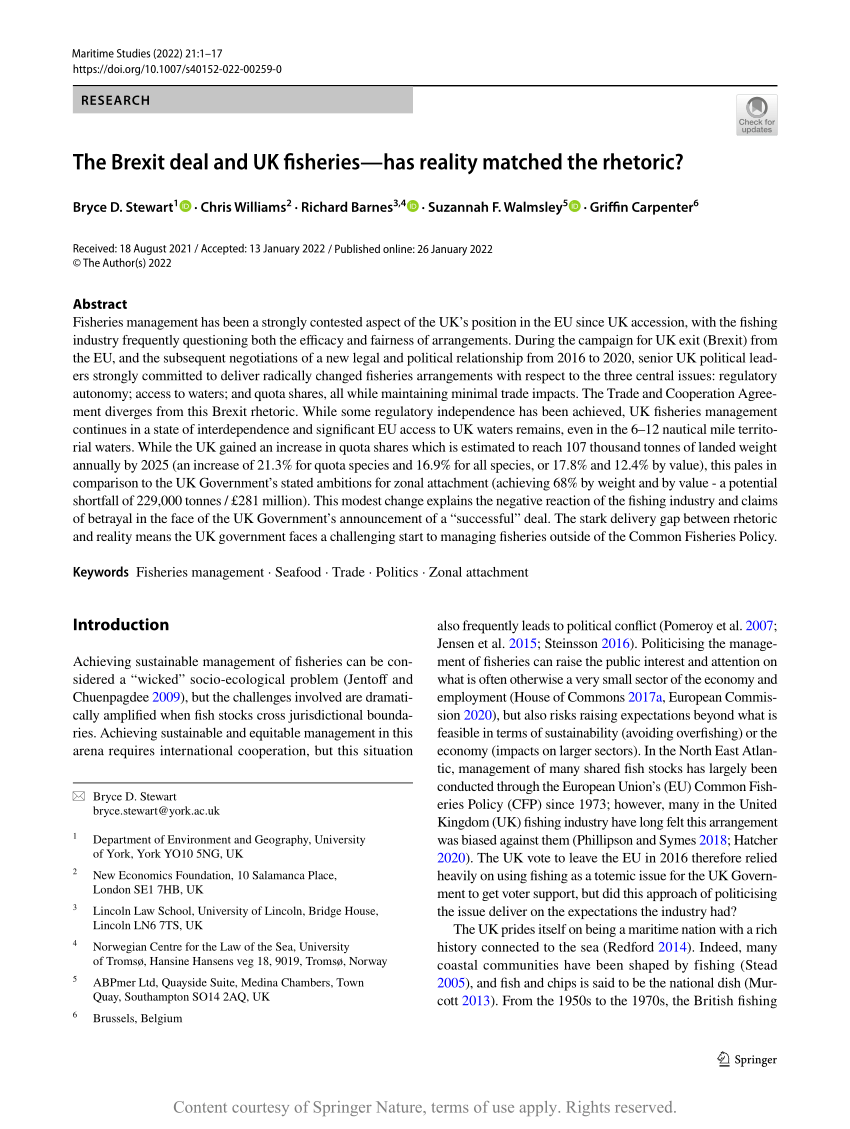
\includegraphics{_images/brexit} \end{center}

\hypertarget{a-self-serving-plug}{%
\chapter{A self-serving plug}\label{a-self-serving-plug}}

Data reveals all.

\begin{center}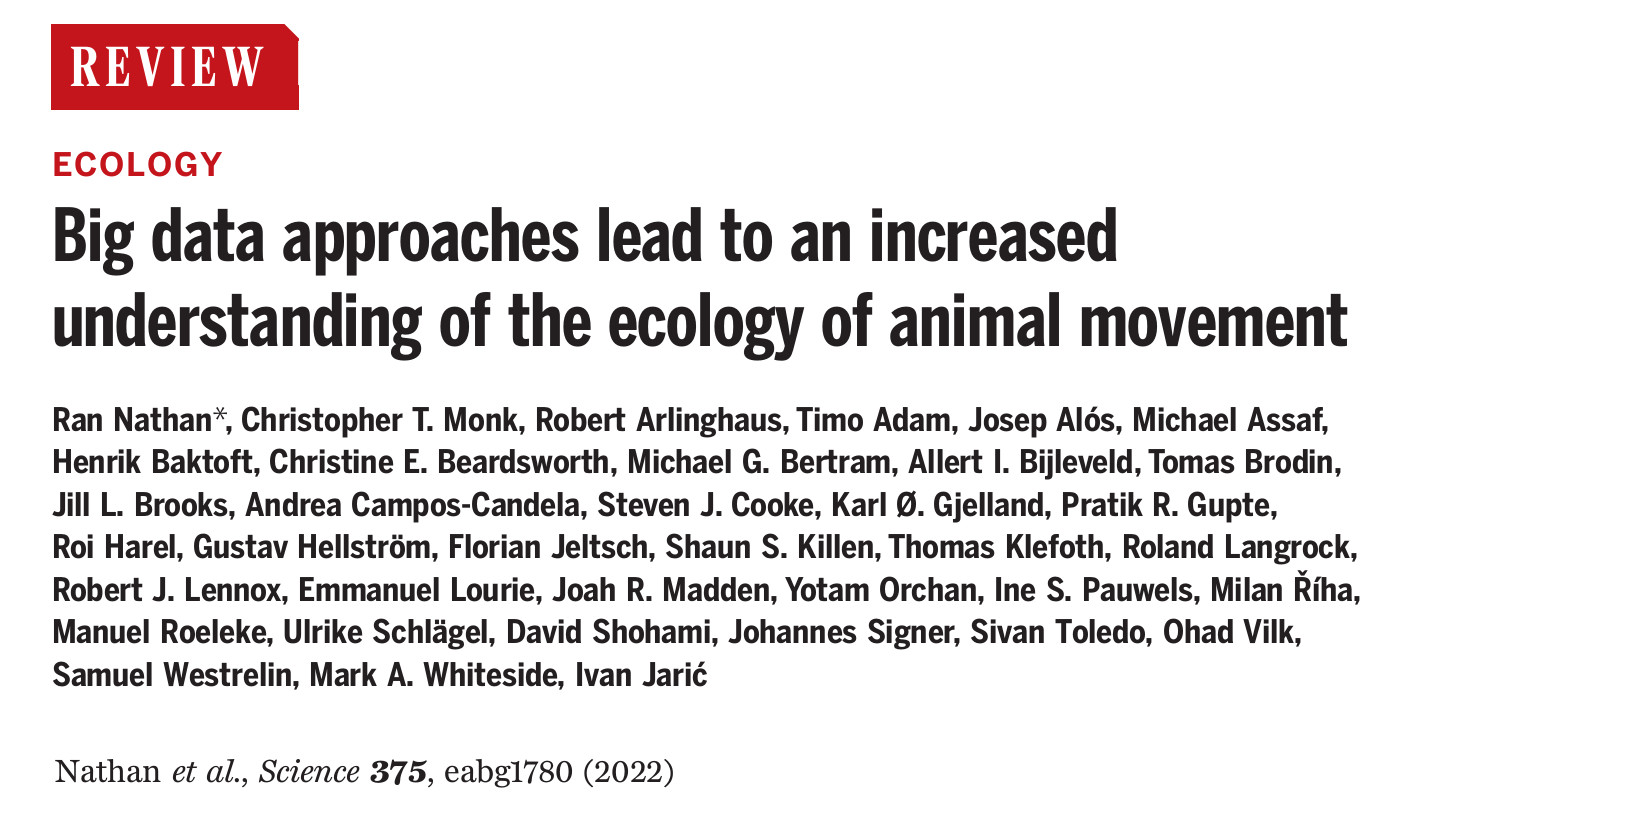
\includegraphics{_images/big} \end{center}

\hypertarget{galapagos-marine-park}{%
\chapter{Galapagos Marine Park}\label{galapagos-marine-park}}

Rubber meets road.

\begin{center}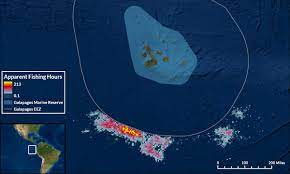
\includegraphics{_images/chinese} \end{center}

\hypertarget{next-chapter}{%
\chapter{Next chapter}\label{next-chapter}}

Where does this take you? (and me?)

  \bibliography{book.bib,packages.bib}

\end{document}
